\documentclass{bachelor_report}

% Додаткові пакети вносіть у цей файл
\input{01_packages}
\addbibresource{../BIB/Resources.bib}

% Додаткові визначення та перевизначення команд вносіть у цей файл
\input{02_redefinitions}

% Відомості про автора роботи
\input{03_data}

% Встановлення числового представлення розділів
\renewcommand{\thesection}{\arabic{section}}

% Встановлення числового представлення підрозділів
\renewcommand{\thesubsection}{\thesection. \arabic{subsection}}

% Налаштування розділів
\titleformat{\section}
{\normalfont\LARGE\bfseries}{\thesection}{1em}{}

% Налаштування підрозділів
\titleformat{\subsection}
{\normalfont\Large\bfseries}{\thesubsection}{1em}{}

% Починаємо верстку документа
\begin{document}

\setfontsize{12}
\linespread{1}

% Створюємо титульну сторінку
% Титульный лист
\thispagestyle{empty}

\begin{center}
НАЦІОНАЛЬНИЙ ТЕХНІЧНИЙ УНІВЕРСИТЕТ УКРАЇНИ \par
<<КИЇВСЬКИЙ ПОЛІТЕХНІЧНИЙ ІНСТИТУТ ім. Ігоря СІКОРСЬКОГО>>\par
ФІЗИКО-ТЕХНІЧНИЙ ІНСТИТУТ\par

\vspace{7mm}
\begin{figure}[!h]
    \centering
    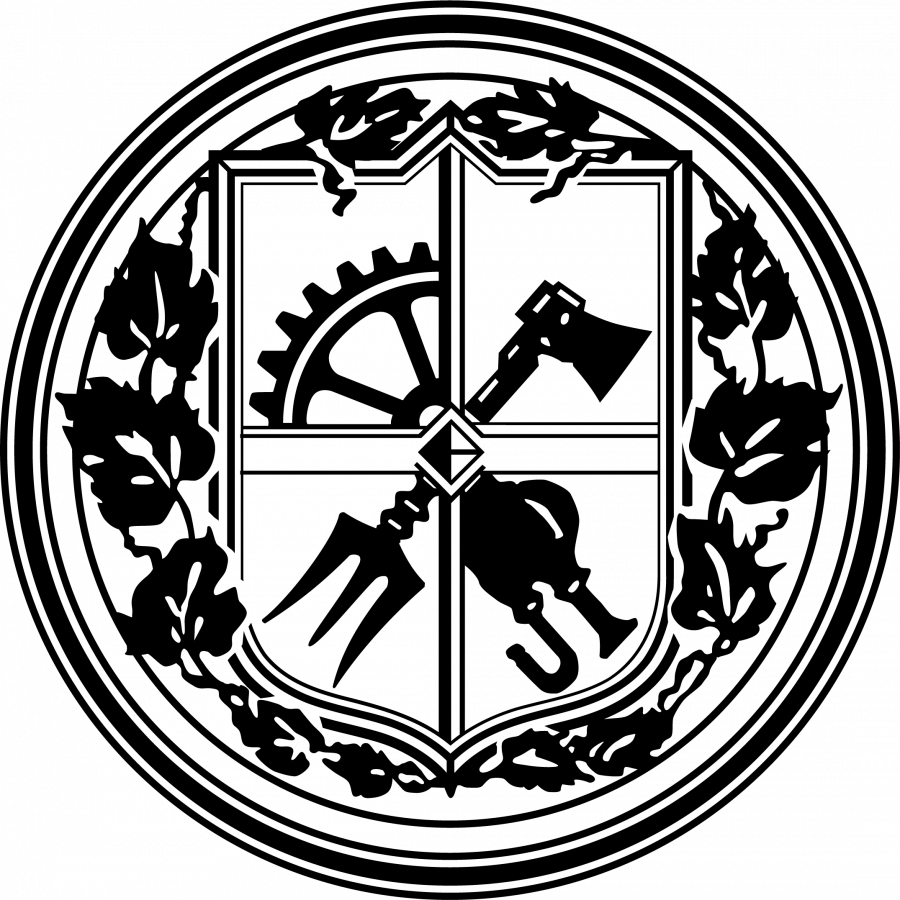
\includegraphics[scale = 0.25]{IMAGES/logoKPI.png}
    \label{logoKPI}
\end{figure}

\vspace{7mm}
{\huge Звіт за темою: \par}
\vspace{1mm}
\LARGE\MakeUppercase{\textbf{\reportTitle}} \par
\end{center}

\vspace{40mm}
\begin{flushright}
Виконали: 

студенти групи \reportAuthorGroup

\reportAuthor

\vspace{20mm}
% Науковий керівник:

% \supervisorRegalia

% \supervisorFio

\end{flushright}

\vspace{10mm}
\begin{center}
{Київ~--- 2023}
\end{center}

\newpage


%% Створюємо зміст    % -- розкоментуйте, якщо зміст вам потрібен
%\pagenumbering{gobble}
\tableofcontents
\cleardoublepage
%\pagenumbering{arabic}

\setcounter{page}{2}    %!!! -- продумати, як автоматизувати номер сторінки

%% Якщо ви використовуєте зміст, то прослідкуйте, щоб номер сторінки 
%% співпадав із справжнім!

% Створюємо вступ
%\intro
%!TEX root = ../thesis.tex
% створюємо вступ

% \setcounter{chapter}{1}
% \setcounter{section}{1}
\vspace{-0.5cm}
\section{Мета практикуму}
Дослідити особливості реалiзацiї сучасних алгебраїчних криптосистем на прикладi учасникiв першого раунду процесу стандартизацiї постквантової криптографiї (NIST PQC).

\subsection{Постановка задачі та варіант завдання}
\vspace{-0.5cm}
\hspace{1cm} \textit{Бригада №4 \textbf{Алгоритм LUOV}}

\vspace{0.5cm}
\begin{tabularx}{\textwidth}{X|X}
	\textbf{Треба виконати} & \textbf{Зроблено} \\
	Детальний опис алгоритму та його складових & \checkmark \\
	Результати порівняльного аналізу з іншими алгоритмами & \checkmark \\
	Огляд наявних результатів досліджень алгоритму & \checkmark  \\
        Результати порівняльного аналізу стійкоті з іншими алгоритмами з можливим застосуванням відомих атак & \checkmark  \\
        Опис власних тестiв, якi проводилися з метою перевiрки коректностi реалiзованої програми & \checkmark  \\
        Детальний опис особливостей реалiзацiї та приклади застосування і тестів & \checkmark  \\
        Результати аналiзу постквантової стiйкостi за наявними результатами аналiзу & \checkmark  \\
\end{tabularx}

% \setcounter{chapter}{2}
% \setcounter{section}{0}

% \section{Результати дослідження}

% Додаємо глави
% Якщо ваша робота містить менше або більше глав - модифікуйте наступні 
% рядки відповідним чином
\section{Хід роботи та опис труднощів}

Для початку було проаналізовано документацію щодо роботи алгоритму LUOV, аналізу проведених атак на даний алгоритм та вiдомих результататів
дослiджень. В процесі роботи було детально описано:
\begin{itemize}
    \item криптографiчний алгоритм LUOV та його складові частини;
    \item реалiзацiї основних алгебраїчних операцiй, якi використовує даний алгоритм;
    \item результати порiвняльного аналiзу швидкодiї даного алгоритму зi схожими алгоритмами (або модифiкацiями алгоритму за допомогою замiни складових частин);
    \item наявні результати дослiджень даного алгоритму;
    \item результати порiвняльного аналiзу стiйкостi даного алгоритму зi схожими алгоритмами з обґрунтуванням можливостi застосування вiдомих атак
    \item власні тести, які проводились для перевірки коректності реалізованого алгоритму
    \item особливості реалізації
    \item результати аналізу постквантової стійкості алгоритму LUOV.
\end{itemize}

В результаті було отримано повний теоретичний опис алгоритму та реалiзацiї основних алгебраїчних операцiй, якi використовує обраний алгоритм. Дані описи будуть використовуватись безпосередньо для подальшої реалізації даного алгоритму.

При виконанні практикуму ніяких труднощів не виникло.

% виникли невеликі труднощі з ..., через що було прийнято рішення ...

%!TEX root = ../thesis.tex

\section{Результати дослідження}
\label{chap:research_results} 

В результаті проробленої роботи було детально проаналізовано та теоретично описано алгоритм LUOV та реалiзацiї основних алгебраїчних операцiй, якi використовує даний алгоритм.

\subsection{Опис алгоритму}

\textbf{LUOV Signature Scheme for NIST PQC Project} --- це пост--квантовий алгоритм цифрового підпису, заснований на використанні еліптичних кривих. Він забезпечує безпеку підпису навіть у випадку, якщо квантові комп’ютери будуть створені.

Алгоритм LUOV Signature Scheme є одним із найперспективніших пост--квантових алгоритмів цифрового підпису. Він є безпечним, ефективним і відносно простим у реалізації.

LUOV = UOV + PRNG + Field Lifting + спрощений секретний ключ, де:
\begin{itemize}
    \item UOV -- одна з найстаріших і найкраще вивчених схем підпису в галузі багатоваріантної криптографії. Вона була розроблена Дж. Патаріном у 1997 році та витримала два десятиліття криптоаналізу. Схема UOV дуже проста, має маленькі підписи та швидка. Однак основним недоліком UOV є те, що відкритий ключ досить великий. LUOV покращує UOV, щоб прискорити алгоритм і зменшити розмір відкритого ключа.
    \item PRNG -- у оригінальній схемі UOV спочатку навмання вибирається секретний ключ, а потім обчислюється відповідний відкритий ключ. Однак також можна випадково вибрати велику частину відкритого ключа, а потім обчислити відповідний секретний ключ і решту відкритого ключа. LUOV використовує цю техніку, так що більша частина відкритого ключа може бути згенерована з PRNG. Це значно зменшує розмір відкритого ключа.
    \item Field Lifting -- LUOV генерує пару ключів над бінарним полем F2, але підносить ці ключі до розширення поля (наприклад, F 27,F247), щоб використовувати їх для підпису та перевірки повідомлень. Це значно зменшує розмір ключів (оскільки кожен коефіцієнт є одним бітом), але не впливає на складність розв’язування системи поліномів, оскільки розв’язки живуть лише в полі розширення.
    \item Спрощений секретний ключ -- UOV, як і багато інших схем MQ, має властивість, що секретний ключ не є унікальним. Існує величезна кількість секретних ключів, які можуть відповідати одному відкритому ключу. Однак не всі ці можливі секретні ключі однаково ефективні. LUOV вибирає певний секретний ключ, щоб генерація та підписання ключів відбувалися набагато швидше.
\end{itemize}

% \vspace{0.5cm}
Алгоритм LUOV використовує функції розширюваного виведення SHAKE для надання криптографічно захищених псевдовипадкових потоків бітів.

\textbf{Приватний ключ для схеми підпису LUOV} -- це послідовність із 256 випадкових бітів (які використовуються для заповнення Keccak1600 Sponge) і просто кодується як послідовність із 32 байтів.

\textbf{Відкритий ключ схеми підпису LUOV} -- це послідовність із 32 байтів (які використовуються для заповнення Keccak Sponge) і матриці $m$ на $\frac{m(m+1)}{2}$ із двійковими записами. Матриця кодується шляхом об’єднання стовпців і доповнення результату нульовими бітами, щоб отримати послідовність бітів, довжина яких ділиться на $8$. Потім послідовність інтерпретується як послідовність байтів, де перші біти мають найменші значення.

\textbf{Публічне початкове число}, представлене 32 байтами, отримують із губки шляхом стиснення (видавлювання) 32 байтів.

\textbf{Губка (sponge)} --- це криптографічна геш-функція з деревоподібною структурою, яка дозволяє ефективно абсорбувати дані та стискати вихід.

В алгоритмі LUOV в якості функції, яка використовує конструкцію губки виступає Keccak1600.

\vspace{0.5cm}
Розглянемо еліптичну криву $E$ над полем $F_p$, де $p$ -- просте число. Нехай $G$ -- точка на кривій $E$, а $n$ -- деяке число, що ділить порядок групи $E(F_p)$.

\vspace{0.25cm}
\textbf{Параметри алгоритму LUOV:}
\begin{itemize}
    \item Еліптична крива (наприклад, $E: y^2 = x^3 + 7x + 5$)
    \item Поле $F_p$ (наприклад, $F_{17}$)
    \item Базова точка G на кривій (наприклад, $G=$(3, 12))
    \item Геш-функція (наприклад, SHAKE-256)
    \item Функція стиснення($sponge$) (наприклад, Keccak) 
\end{itemize}

% \vspace{0.5cm}
\newpage
\textbf{\largeАлгоритм генерації ключів для LUOV}
\vspace{0.25cm}
 \begin{algorithm}
    Генерація ключів для LUOV. \\Вхід: $private_seed$ -- початкове значення для створення ключа. \\Вихід: ($public\_seed, Q_2$) -- публічний ключ, $private\_seed$ -- відповідний закритий ключ.
    % Приймає в якості вхідних даних приватний набір і виробляє відкритий ключ (публічний набір, Q2) і приватний ключ (приватний набір).
    \begin{enumerate}
        \item Ініціалізується губка з заданим $private\_seed$, результатом якої є $private\_sponge$. 
        % $private_sponge = InitializeAndAbsorb(private seed)$
        \item Вичавлюється публічний набір з $private\_sponge$. Публічний набір використовується для отримання відкритого ключа і оприлюднюється.
        % SqueezePublicSeed(private sponge)
        \item Вичавлюється значення $T$ з $private\_sponge$. Значення $T$ використовується для отримання приватного ключа і зберігається в секреті.
        % SqueezeT(private sponge)
        \item Ініціалізується інша губка з $public\_seed$.
        % InitializeAndAbsorb(public seed)
        \item Вичавлюються три значення ($C$, $L$, $Q_1$) з $public\_sponge$. Значення $C$ і $L$ використовуються для отримання відкритого ключа, а значення $Q_1$ використовується для отримання приватного ключа.
        % SqueezePublicMap(public sponge)
        \item Обчислюються значення $Q_2$ з $Q_1$ і $T$. Значення $Q_2$ є частиною відкритого ключа.
        % FindQ2(Q1, T)
        \item В результаті повертається відкритий ключ ($public\_seed$, $Q_2$) і приватний ключ ($private\_seed$).
        % Return (public seed, Q2) and private seed
    \end{enumerate}
\end{algorithm}

Саме функція, яка обчислює значення $Q_2$ -- FindQ2($Q1$, $T$) є важливою частиною алгоритму. Вона забезпечує безпеку алгоритму, оскільки її важко обчислити, знаючи лише значення $Q_1$ і $T$.

\vspace{0.25cm}
\textbf{\largeАлгоритм генерування підпису LUOV}
\vspace{0.25cm}
\begin{algorithm}
    LUOV Signature Scheme працює наступним чином: \\
    Вхід: відкритий ключ ($s_1$,$s_2$), приватний ключ $private\_seed$, повідомлення $M$. \\
    Вихід: підпис $s$.
    \begin{enumerate}
        \item Ініціалізація губки до нульового стану та поглинання даних з $private\_seed$. В результаті отримуємо значення sponge.
        \item Вичавлювання значення $public\_seed$ з sponge.
        \item Обчислення значення $T$ зі sponge.
        \item Ініціалізація губки до нульового стану та поглинання даних з $public\_seed$. В результаті отримуємо значення $public\_sponge$.
        \item Обчислення значень матриць $C$, $L$ і $Q_1$ шляхом відбору колонок з $public\_sponge$.
        \item Ініціалізація губки до нульового стану та поглинання даних з конкатенації повідомлення $M$ та його падінгу $0x00$. В результаті отримуємо значення $hash\_sponge$ для гешування повідомлення.
        \item Обчислення геш-значення повідомлення $M$ з $hash\_sponge$. В результаті отримуємо вектор геш-значень $h$.
        \item Ініціалізація губки до нульового стану та поглинання даних з конкатенації повідомлення $M$, його падінгу $0x00$ та значення $private\_seed$. В результаті отримуємо губку з випадковими числами $vinegar\_sponge$ для генерування підпису.
        \item Поки не знайдено такого $s'$, яке задовольнить рівняння $F(s')$ = $h$, виконуємо наступний цикл:
        \begin{enumerate}
            \item Вичавлювання байтів з губки $vinegar\_sponge$ та їх інтерпретація в кодування. В результаті отримуємо вектор $v$.
            \item Побудова розширеної матриці $A$ для лінійної системи $F(v||o)$ = $h$. Для побудови беруться в якості вхідних даних $C$, $L$, $Q_1$, $T$, $h$, $v$. В результаті отримуємо значення матриці $A$ -- розв'язку лінійної системи методом Гауса.
            \item Якщо система $F(v||o)$ = $h$ має унікальне рішення $o$, то: $s'$ = $(v||o)^T$.
        \end{enumerate}
        \item Обраховуємо значення $s$: 
            $s = \begin{pmatrix}
            1_v & -T \\
            0 & 1_m
            \end{pmatrix} \cdot s'$
        \item Повернення значення підпису $s$.
    \end{enumerate}
\end{algorithm}

\newpage
\textbf{\largeАлгоритм верифікації підпису LUOV\\}
\vspace{-0.5cm}
\begin{algorithm}{
Верифікація підпису LUOV.\\
Вхід: ($public\_seed$,$Q_2$) -- публічний ключ, повідомлення $M$, підпис $s$. \\
Вихід: \textit{Прийнято (accept)} - якщо підпис $s$ дійсний, \textit{Відхилено (reject)} - в інших випадках.
\begin{enumerate}
    \item Ініціалізація губки до нульового стану та поглинання даних з конкатенації повідомлення $M$ та його падінгу 0x00. В результаті отримуємо губку $sponge$ для гешування.
    \item Обчислення геш-значення повідомлення $M$ з губки $sponge$. В результаті отримуємо вектор геш-значень $h$.
    \item За алгоритмом EvaluatePublicMap перевіряє підпис за вхідними даними $(public\_seed, Q_2)$ та $s$.
    \begin{enumerate}
        \item якщо значення $e$ та $h$ співпадають: алгоритм повертає \textit{Accept}
        \item в іншому випадку: алгортм повертає \textit{Reject}.
    \end{enumerate}
\end{enumerate}}
\end{algorithm}

Також схема підпису може використовуватись в \textbf{режимі відновлення повідомлень}. Використання відновлення повідомлення не впливає на алгоритм створення підпису. Ту саму пару ключів можна використовувати для підпису повідомлень у обох режимах підпису. Підпис для $M$ у режимі доданого підпису не пов’язаний з підписом для того самого повідомлення в режимі відновлення повідомлення, оскільки інший байт додається до повідомлення в кожному режимі.

\textbf{Безпека алгоритму:} \\
Безпека алгоритму LUOV Signature Scheme базується на тому, що важко обчислити точку $P$, знаючи лише точку $Q$ і пару чисел $(a,b)$. Ця задача є $NP$--складною, і навіть якщо квантові комп’ютери будуть створені, то її рішення буде вимагати значних ресурсів.

\textbf{Основні алгебраїчні операції, які використовує LUOV:}
\begin{itemize}
    \item Додавання еліптичних кривих:
    \begin{equation}
    Q = aP + bG
    \end{equation}
    \item Множення числа на точку еліптичної кривої:
    \begin{equation}
    s_1Q = aP + bGs_1
    \end{equation}
\end{itemize}

\subsection{Продуктивність LUOV}
\vspace{-0.5cm}
\begin{table}[h!]
    \centering
    \begin{tabular}{|p{1,3cm}|p{2cm}|p{2cm}|p{1,3cm}|p{2cm}|p{2cm}|p{2,1cm}|}
        \hline
       \textbf{Рівень безпеки} & \textbf{Розмір секретного ключа} & \textbf{Розмір відкритого ключа} & \textbf{Розмір підпису} & \textbf{Генерація ключів} & \textbf{Підписання} & \textbf{Перевірка} \\
        \hline
       \centering 1 & \centering 32 Б & \centering 11,5 Кб & \centering 239 Б & 1,1 М циклів & 224 К цикли & 49 К циклів \\
        \hline
       \centering 3 & \centering 32 Б & \centering 35,4 Кб & \centering 337 Б & 4,6 М циклів & 643 К цикли & 152 К цикли \\
        \hline
       \centering 5 & \centering 32 Б & \centering 82,0 КБ & \centering 440 Б & 9,7 М циклів & 1,1 М циклів & 331 К циклів \\
        \hline
    \end{tabular}
    \caption{\large Характеристики продуктивності оптимізованої реалізації LUOV}
    \label{tab:security_levels}
\end{table}

Характеристики продуктивності оптимізованої реалізації LUOV з постійним часом AVX2. Для покращення продуктивності дана реалізація виконує деякі попередні обчислення пари ключів. Для впровадження без інструкцій AVX2 або з різними рівнями попереднього обчислення звертаємося до документа NIST PQC Round2.

\subsection{Атака QuantumHammer}

Схема Oil and Vinegar є однією з найкраще вивчених багатоваріантних схем підпису, яка, за умови правильного вибору параметрів, витримує всі криптоаналізи з 1997 року.

Гібридна атака QuantumHammer --- це комбінація двох атак: атаки трасування бітів, увімкненої за допомогою впровадження помилки Rowhammer, і атаки розділяй і володарюй, яка використовує трасування бітів як оракул. Використовуючи трасування бітів, зловмисник, маючи доступ до помилкових підписів, зібраних за допомогою атаки Rowhammer, може відновити секретні ключові біти, хоча й повільно. Використовується атака «розділяй і володарюй», яка в свою чергу використовує структуру в частині LUOV, яка генерує ключі, і ефективніше розв’язує систему рівнянь для секретного ключа з кількома бітами ключа, відновленими за допомогою трасування бітів. Було продемонстровано першу успішну атаку в дикій природі на LUOV, яка відновила всі 11 тисяч бітів ключа менш ніж за 4 години активної атаки Rowhammer. Частина постобробки є дуже паралельною, тому її можна тривіально пришвидшити, використовуючи скромні ресурси. QuantumHammer не робить жодних нереалістичних припущень, вимагає лише спільного розміщення програмного забезпечення (без фізичного доступу), і тому може використовуватися для націлювання на спільні хмарні сервери або в інших середовищах ізольованого програмного середовища.

Таким чином атака Rowhammer може призвести до серйозних наслідків через перевертання бітів в інших процесах і витік ключової інформації. QuantumHammerattack поєднує в собі обидві слабкі сторони, щоб розпочати успішну атаку з відновленням повного секретного ключа схеми.

\subsection{Атака Nested Subset Differential Attack}

Модифікована версія диференціальної атаки підполя під назвою «Вкладена диференціальна атака підмножини» повністю порушує половину параметрів, встановлених у раунді 2 версії Lifted Unbalanced Oil and Vinegar. Автори звели атаку на ці набори параметрів до проблеми розв’язання квадратних рівнянь над простим полем F2. Це робить їхню атаку достатньо ефективною для практичного виконання. Оскільки дана атака не використовувала незбалансовану структуру LUOV, її можна розглядати як метод вирішення піднятих квадратичних систем загалом. Автори вважають, що необхідні додаткові дослідження для розв’язання такого типу квадратичних систем за допомогою атаки NSDA. Також було проведено експериментальні атаки на фактичні параметри LUOV і змогли підробити підпис менш ніж за 210 хвилин.

Також на алгоритм підпису LUOV проводились такі "класичні атаки" як DirectAttack та HashCollisionAttack.

\subsection{Опис власних тестiв}

Для реалізації алгоритму LUOV проводились наступні тести:

\begin{itemize}[label={$\bullet$}]
    \item Тест на швидкодію в залежності від розміру вхідного повідомлення. \\
    Для тесту використовувались повідомлення різних розмірів (100 символів, 1000 символів та 10000 символів). В результаті було отримано, що швидкодія підписання та перевірки підпису не залежить від довжини вхідного повідомлення. Середня швидкодія при виконанні даного тесту лежить в межах проміжку [600,900] мс.
    \item Тест генерації підпису. \\
    В результаті було отримано правильний підпис для повідомлення.
    \item Тест верифікації підпису повідомлення. \\
    В результаті було отримано значення true після верифікації підпису для повідомлення.
    \item Тест верифікації пошкодженого повідомлення. \\
    В результаті було отримано значення false після верифікації підпису для пошкодженого повідомлення.
    \item Тест використання різних параметрів кривої.
    В результаті було показано використання алгоритму підпису LUOV для 2-ох можливих варіантів набору параметрів.
\end{itemize}

\subsection{Детальний опис особливостей реалiзацiї та приклади застосування}

При реалізації алгориму цифрового підпису LUOV посилалися на деякі інші відомі реалізації алгоритму, включно з документацією. Ось деякі з них:
\begin{enumerate}
    \item \url{https://github.com/WardBeullens/LUOV}
    \item \url{https://github.com/saadislamm/QuantumHammer}
    \item \url{https://github.com/Danny-xyy/LUOV}
    \item \url{https://github.com/EddAngulo/luov_java_implementation}
    \item \url{https://github.com/WardBeullens/ThesisCode}
\end{enumerate}

\vspace{0.5cm}
\textbf{Основні функції реалізації алгоритму}:
\begin{enumerate}
    \item Можливість вибору поля з параметрами для роботи з алгоритмом серед запропонованих:
    \begin{itemize}
        \item GF(207): r=7,m=57,v=197.
        \item GF(261): r=61,m=60,v=261.
    \end{itemize}
    \item Функція генерації публічного та приватного ключів: keyGen().
    \item Функція генерації підпису повідомлення: sign().
    \item Функція перевірки підписаного повідомлення: verify(). 
\end{enumerate}

\vspace{0.5cm}
\textbf{\LargeПриклади використання реалізації та проведених тестів:}

% \vspace{-0.5cm}
\begin{figure}[ht]
    \centering
    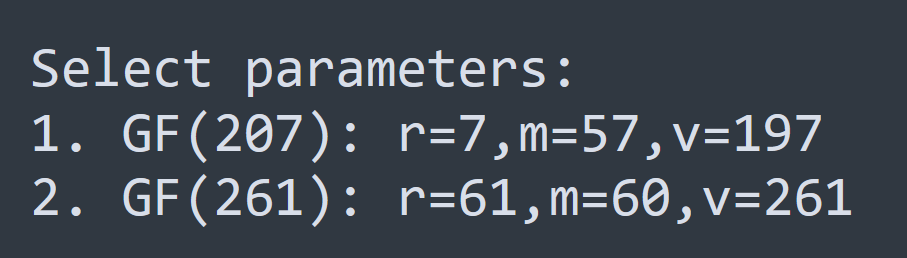
\includegraphics[scale = 0.55]{IMAGES/select_parameters.png}
    \caption{Можливість вибору параметрів.}
    \label{fig1}
\end{figure}

\begin{figure}[ht]
    \centering
    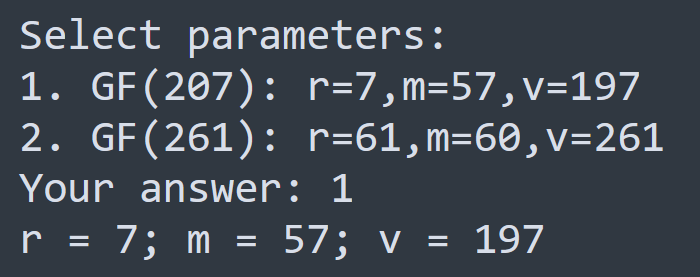
\includegraphics[scale = 0.7]{IMAGES/select_param1.png}
    \caption{Вибір 1-го типу параметрів.}
    \label{fig1}
\end{figure}

\begin{figure}[ht]
    \centering
    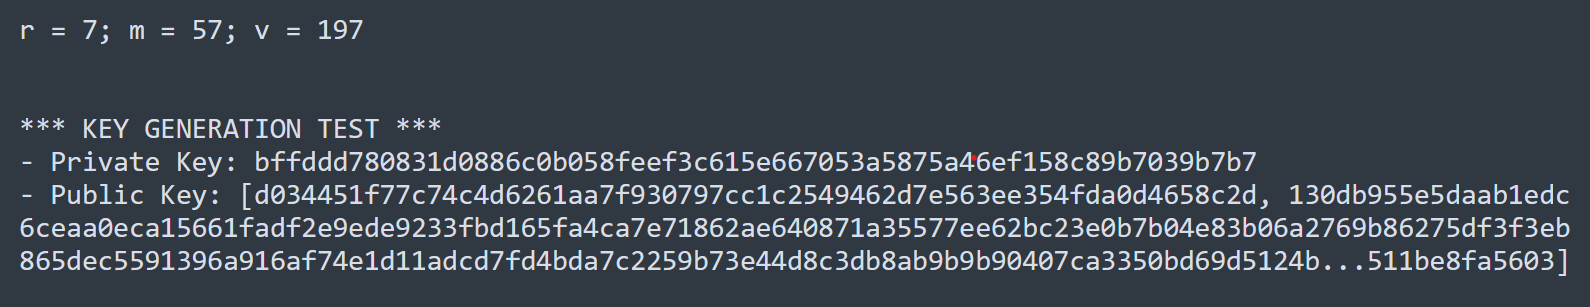
\includegraphics[scale = 0.6]{IMAGES/key_gen1.png}
    \caption{Генерація ключів для 1-го типу параметрів.}
    \label{fig1}
\end{figure}

\begin{figure}[ht]
    \centering
    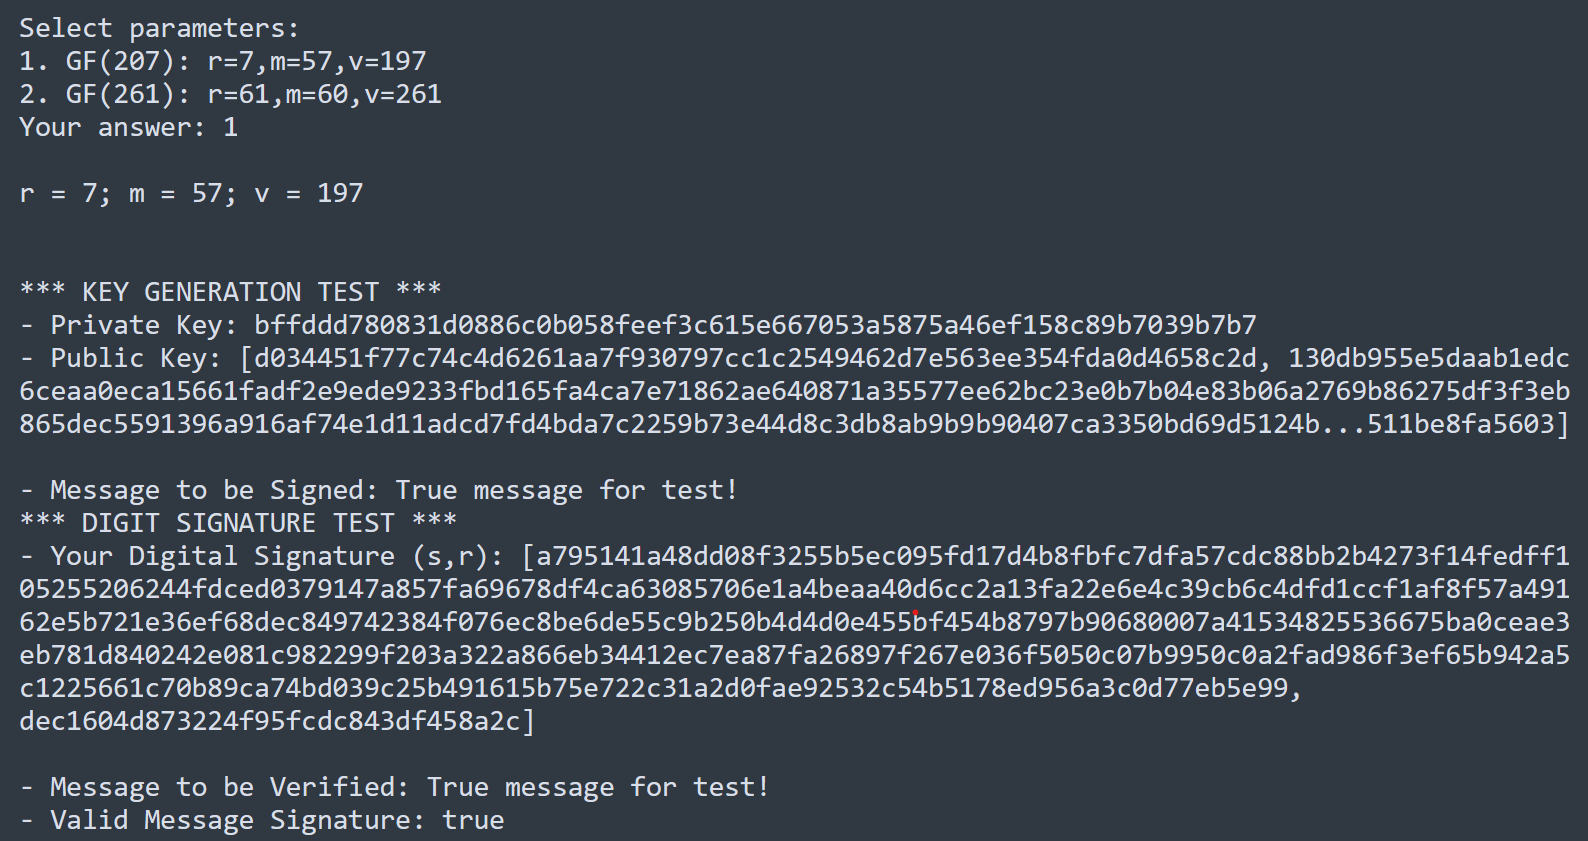
\includegraphics[scale = 0.53]{IMAGES/digit_sign_testT1.png}
    \caption{\largeПідписування повідомлення для 1-го типу параметрів.}
    \label{fig1}
\end{figure}
% \vspace{2cm}
\begin{figure}[ht]
    \centering
    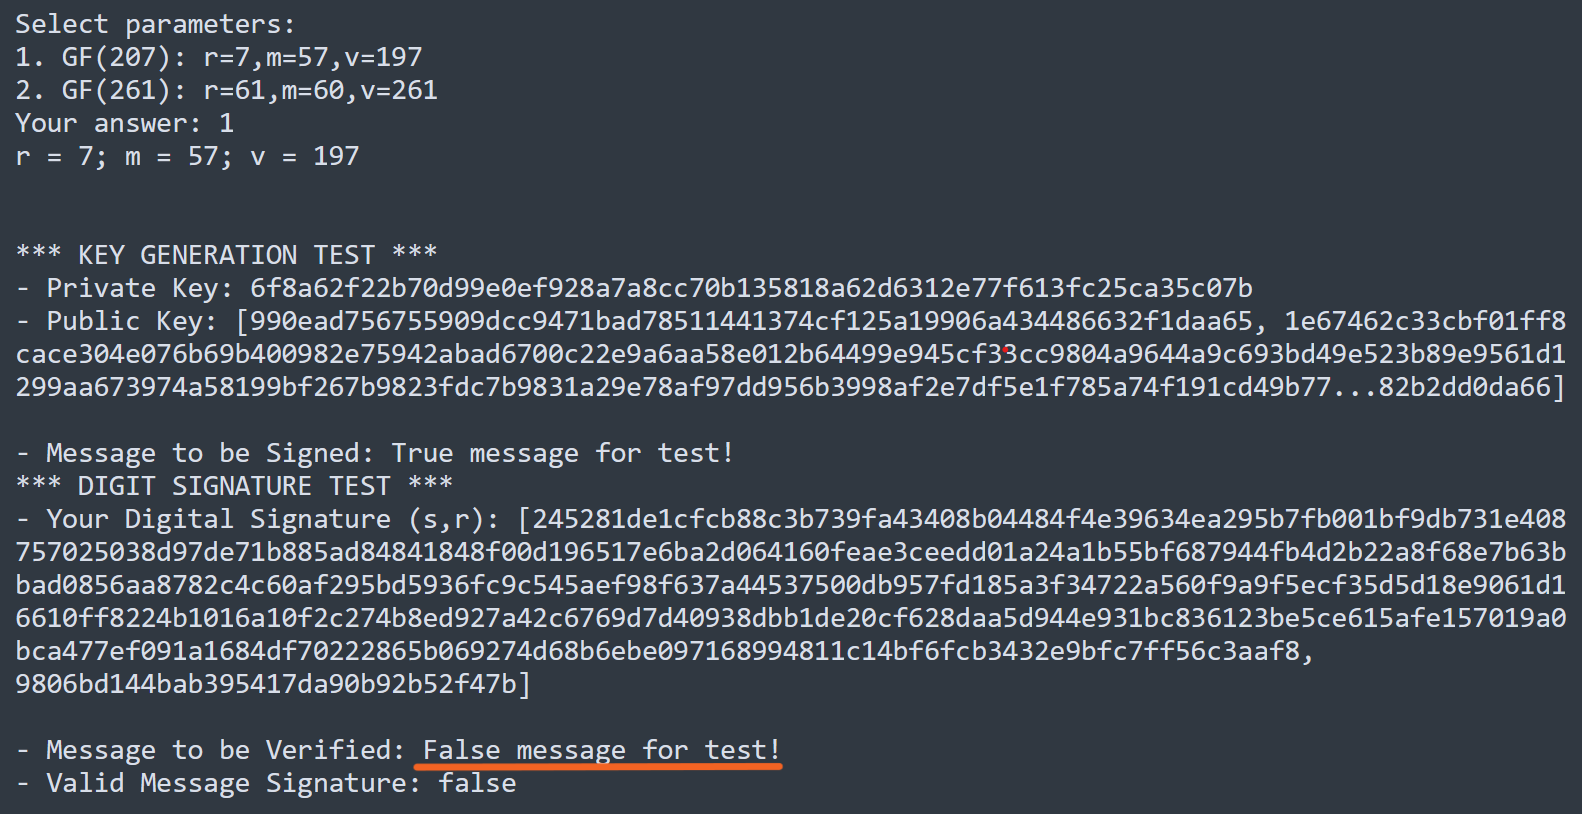
\includegraphics[scale = 0.53]{IMAGES/digit_sign_testF1.png}
    \caption{\largeПошкодження повідомлення при верифікації для 1-го типу параметрів.}
    \label{fig1}
\end{figure}

\begin{figure}[ht]
    \centering
    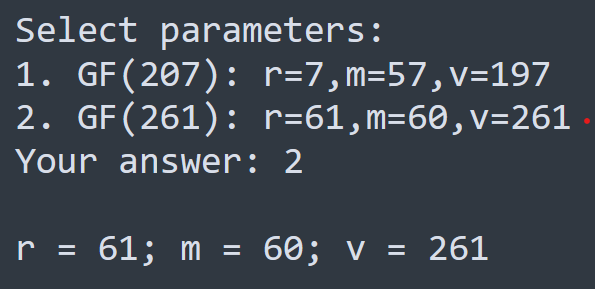
\includegraphics[scale = 0.7]{IMAGES/select_param2.png}
    \caption{Вибір 2-го типу параметрів.}
    \label{fig1}
\end{figure}

\begin{figure}[ht]
    \centering
    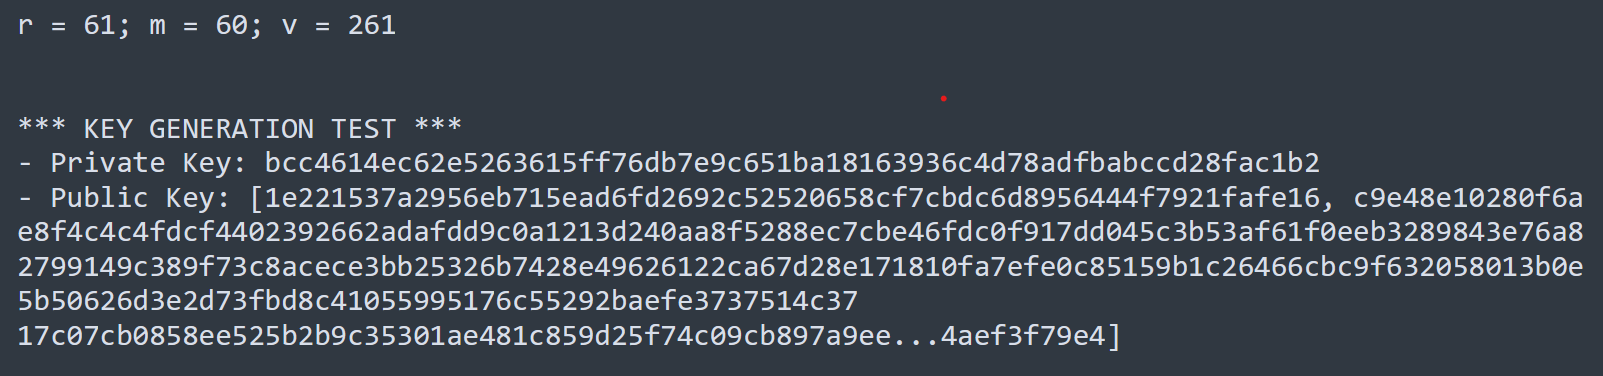
\includegraphics[scale = 0.6]{IMAGES/key_gen2.png}
    \caption{Генерація ключів для 2-го типу параметрів.}
    \label{fig1}
\end{figure}

\begin{figure}[ht!]
    \centering
    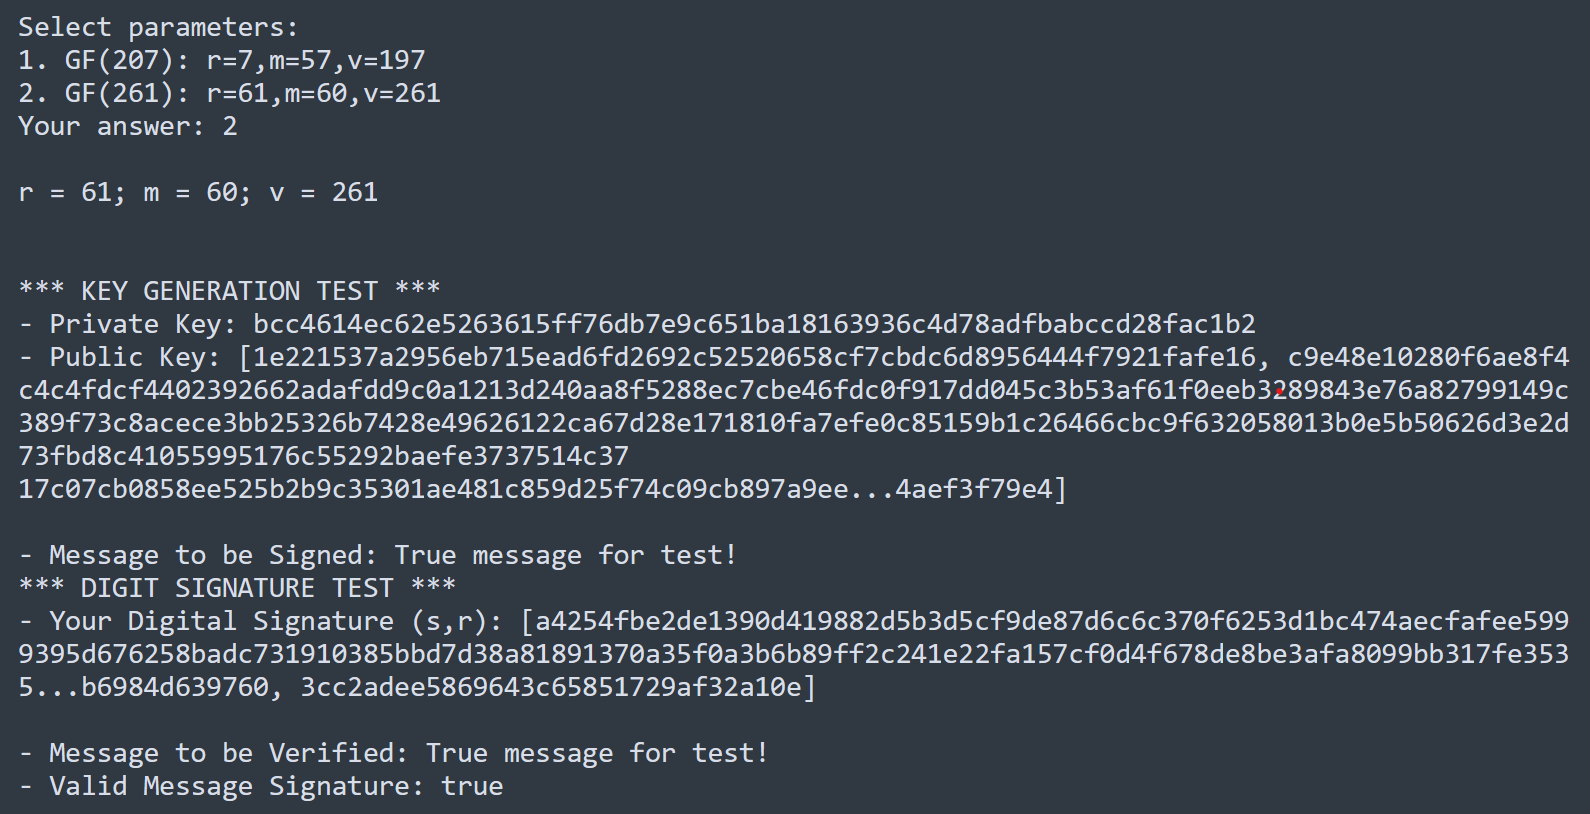
\includegraphics[scale = 0.6]{IMAGES/digit_sign_testT2.png}
    \caption{\largeПідписування повідомлення для 2-го типу параметрів.}
    \label{fig1}
\end{figure}

\newpage
А також прикріплюємо результат тесту верифікації підпису з пошкодженим повідомленням для 2-го типу параметрів кривої:

\begin{figure}[ht!]
    \centering
    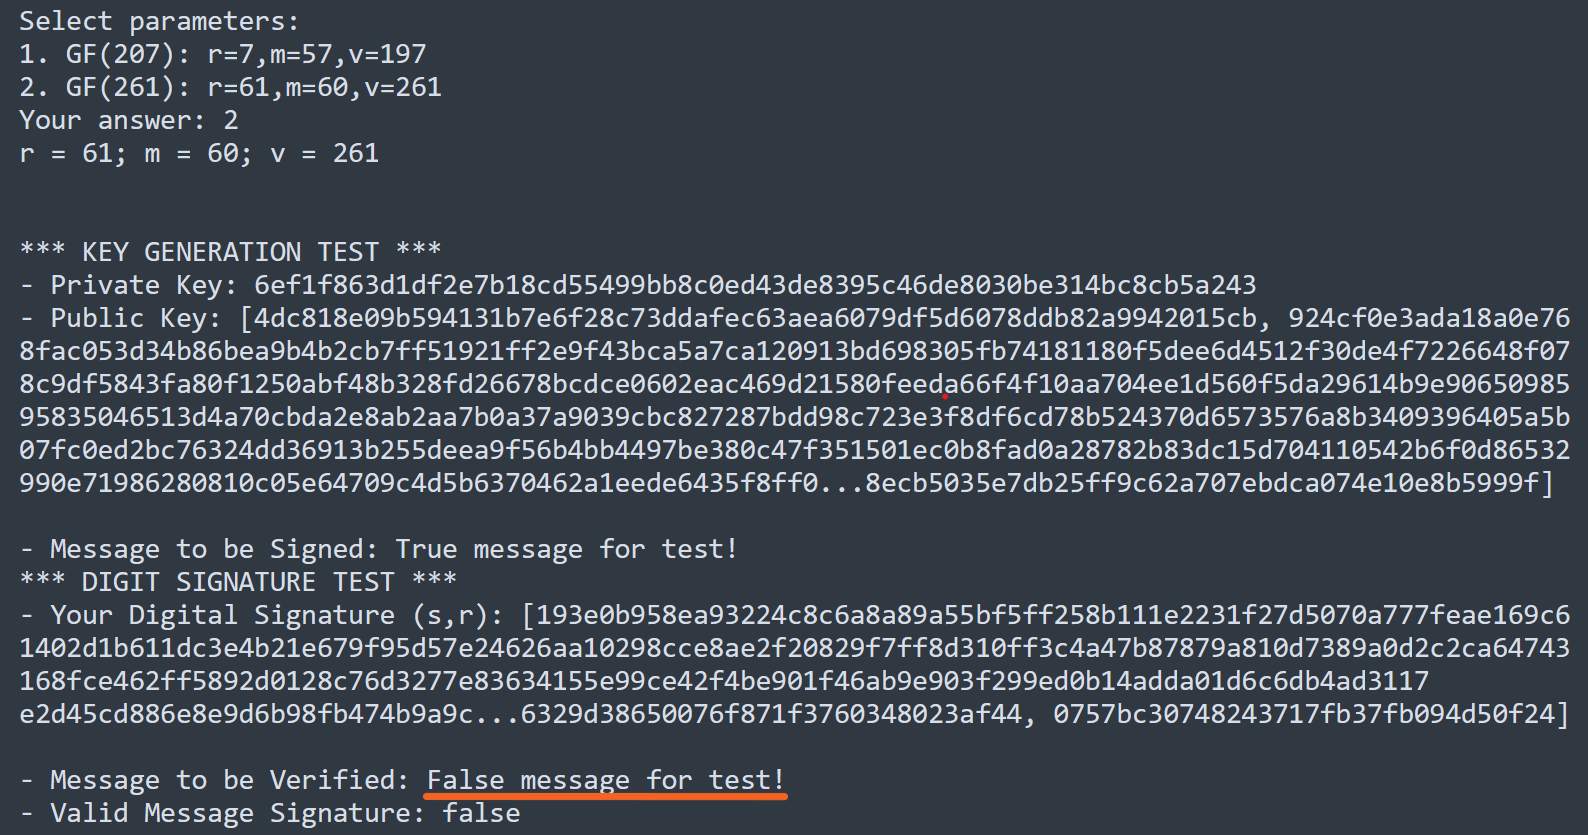
\includegraphics[scale = 0.6]{IMAGES/digit_sign_testF2.png}
    \caption{\largeПошкодження повідомлення при верифікації для 2-го типу параметрів.}
    \label{fig1}
\end{figure}

\newpage
\subsection{Результати аналiзу постквантової стiйкостi}
\vspace{-0.5cm}
Постквантову стійкість можна перевірити оцінкою складності прямої атаки на LUOV з одним з можливих наборів параметрів, наприклад (r = 7, m = 57, v = 197); можемо визначити рівень безпеки, який досягає цей набір. Для цього можна скористатися використанням методу Тома і Вольфа. Таким чином можна звести пошук розв'язку цієї недовизначеної системи до пошуку розв'язку детермінованої системи з $57+1-\lfloor(57+197)/57\rfloor$ = 54 рівняння. Ми припускаємо, що ця система та системи, отримані шляхом фіксації ряду змінних, є напіврегулярними. Якщо ми фіксуємо k додаткових змінних, то ступінь регулярності дорівнює ступеню першого члена в степеневому ряді:

$S_{54,54-k}(x) = \frac{(1-x^2)^{54}}{(1-x)^{54-k}}$, який має недодатний коефіцієнт.\\
Для k = 0 ми маємо $S_{54}(x)$ = $(1 + x)54$, тому ступінь регулярності дорівнює 55.
Продовжуючи обчислення далі визначимо, що складність прямої атаки перевищує нижню межу 2146×1,1, як вимагається.
А якщо використати пошук Гровера замість частини гібридного підходу грубої сили, щоб прискорити пряму атаку. Таким чином продовжуючи обчислення далі дійдемо до того, що для всіх вибраних параметрів і всіх практичних значень k складність навіть одного обчислення базису Гробнера перевищує 264, і алгоритм Гровера повинен виконувати велику кількість цих обчислень послідовно, щоб отримати помітне прискорення порівняно з класичним грубим методом. 

В результаті отримаємо, що алгоритм LUOV має постквантову стійкість до атак.

\newpage
\section{Висновки}

В даному практикумі наведено повний теоретичний опис алгоритму з усiма деталями та вiдомими результатами дослiджень. Проведено теоретичний порiвняльний аналiз обраного алгоритму зi схожими алгоритмами та дослідження вiдомих атак на даний алгоритм. Крім цього в ході практикуму було реалізовано алгоритм LUOV для 2-ох варіантів наборів парметрів кривої. А також проведено власні тести для реалізації алгоритму, проаналізовано постквантову стійкість даного алгоритму. 

% Створюємо висновки
% \conclusions
% \input{../CHAPTERS/w1_conclusions}

% Нарешті
\end{document}